\documentclass[12pt]{article}
\usepackage[top=1in, bottom=1in, left=1in, right=1in]{geometry}

\usepackage{setspace}
\onehalfspacing

\usepackage{amssymb}
%% The amsthm package provides extended theorem environments
\usepackage{amsthm}
\usepackage{epsfig}
\usepackage{times}
\renewcommand{\ttdefault}{cmtt}
\usepackage{amsmath}
\usepackage{graphicx} % for graphics files
\usepackage{tabu}

% Draw figures yourself
\usepackage{tikz} 

% writing elements
%\usepackage{mhchem}

\usepackage{paralist}

% The float package HAS to load before hyperref
\usepackage{float} % for psuedocode formatting
\usepackage{xspace}

% from Denovo Methods Manual
\usepackage{mathrsfs}
\usepackage[mathcal]{euscript}
\usepackage{color}
\usepackage{array}

\usepackage[pdftex]{hyperref}
\usepackage[parfill]{parskip}

% math syntax
\newcommand{\nth}{n\ensuremath{^{\text{th}}} }
\newcommand{\ve}[1]{\ensuremath{\mathbf{#1}}}
\newcommand{\Macro}{\ensuremath{\Sigma}}
\newcommand{\rvec}{\ensuremath{\vec{r}}}
\newcommand{\omvec}{\ensuremath{\hat{\Omega}}}
\newcommand{\vOmega}{\ensuremath{\hat{\Omega}}}
%---------------------------------------------------------------------------
%---------------------------------------------------------------------------
\begin{document}
\begin{center}
{\bf NENG 685, Fa11 2017 \\
Solution Context and Tools\\
October 2, 2017}
\end{center}

\setlength{\unitlength}{1in}
\begin{picture}(6,.1) 
\put(0,0) {\line(1,0){6.25}}         
\end{picture}

We've looked a little bit at the transport equation. To venture much farther in thinking about solving the transport equation, it helps to remember what we're applying it to and some other bits of information that we use. 

As mentioned, we'll mostly focus on defense applications in this class - shielding, detectors, criticality, etc. However, we will sprinkle in a bit about nuclear reactors because they make great examples and you should know a little bit about them as a nuclear engineer. This also allows us to leverage what you are learning now in NENG681 as opposed to material you will learn next quarter in NENG605 and NENG650.

A nuclear reactor is a three-dimensional structure consisting of complicated geometrical shapes made of variety of materials. 	

(switch to ppt for image examples)

\begin{compactitem} 
\item A unit cell usually consists of a fuel rod, gap, cladding and
corresponding moderator. It is usually surrounded by similar
cells. A fuel rod consists of fuel pellets.	

\item A fuel assembly usually consists of several hundred fuel rods
(fuel cells).	

\item A reactor core consists of several hundred fuel assemblies.	

\item Fuel assemblies and fuel rods are usually arranged in square or
hexagonal lattice.	
\end{compactitem}
%
(switch to ppt for image examples)

%-------------------------------------------------------------
%-------------------------------------------------------------
\vspace{-1 em}
\subsection*{Solution Context and Data}%
\begin{figure}[h!]
    \begin{center}
    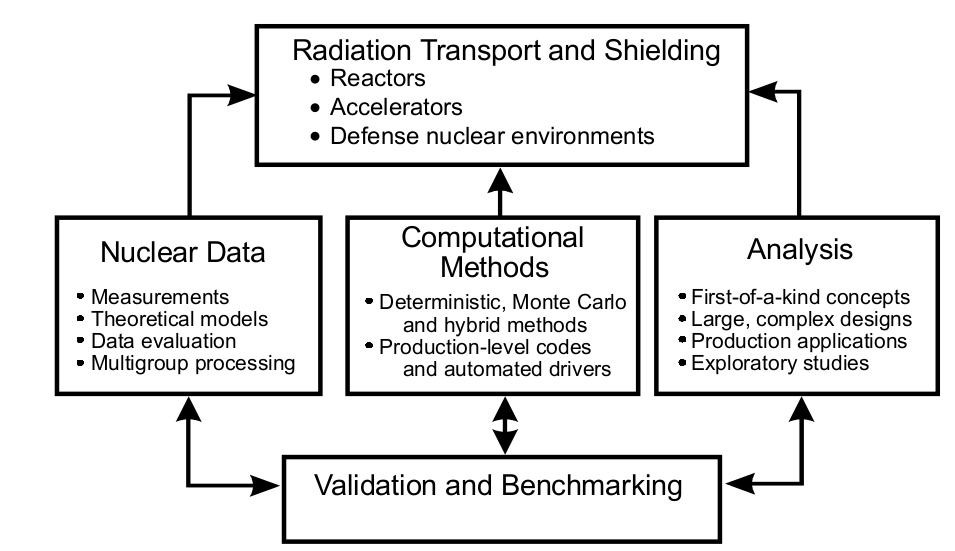
\includegraphics[keepaspectratio, width = 4.5 in]{../figs/solver-map}
    \end{center}
    %\caption{Legendre polynomials}
    \label{fig:context}
\end{figure}
%
We have many different types of geometries and physics going on with the systems we're interested in. However, we take the same fundamental approach no matter what. Each component is incredibly important, but let's take a moment to talk about \textbf{Nuclear Data}.

We need a description of all of the physical interactions happening inside a nuclear reactor that we can use in our equation. An \textit{evaluated nuclear data file} is a collection of various data enabling to reconstruct, for each isotope, its cross-section's 
\begin{compactitem}
\item general information
\item resonance parameters 
\item angular distribution for emitted particles 
\item energy distribution for emitted particles 
\item energy-angle distribution for emitted particles 
\item thermal neutron scattering law data 
\item radioactivity and fission-product yield data 
\item multiplicities for radioactive nuclide production 
\item cross-sections for radioactive nuclide production
\end{compactitem}

There are many evaluations coming from various countries such as: USA, Europe, Japan, Russia, China, \dots Getting from experimental data (what we have of it) + theory (however accurate that is) to data that can actually be used in a code is no small feat. And, that process is sort of a mess...
\begin{figure}[h!]
    \begin{center}
    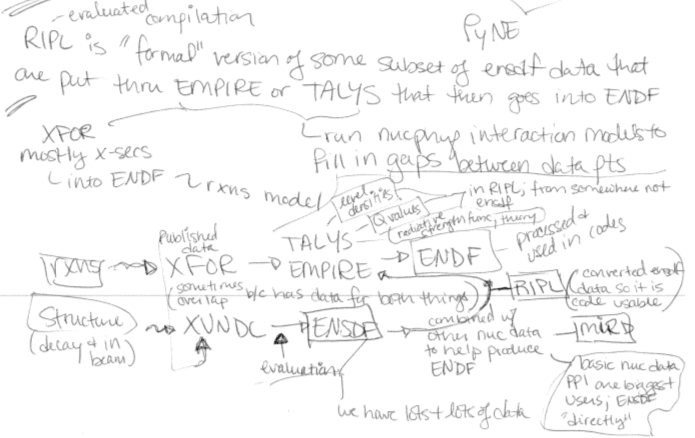
\includegraphics[keepaspectratio, width = 6 in]{../figs/data-notes}
    \end{center}
    \caption{Notes from a meeting where someone tried to explain this to me}
    \label{fig:datanotes}
\end{figure}
\begin{figure}[h!]
    \begin{center}
    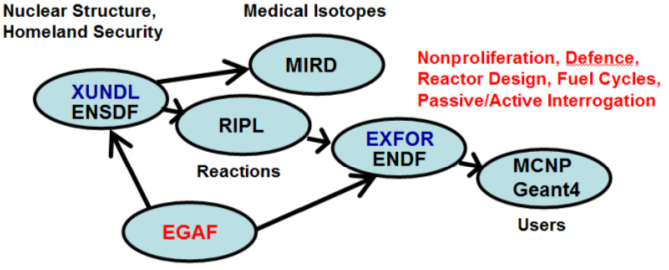
\includegraphics[keepaspectratio, width = 4.5 in]{../figs/hurst-code-map}
    \end{center}
    \caption{A more coherent (but less comprehensive) set}
    \label{fig:hurstfig}
\end{figure}

We won't go through all of this, but I think it's important to have context about what this is and how confusing it can be. There is a lot of data and many formats, it is quite complicated, and can be quite different depending on the application we're interested in. This will be covered in detail in NENG651 (if not - let me know!).  We will also explore aspects of it along the way towards the end of the course.

%-------------------------------------------------------------
%-------------------------------------------------------------
\subsection*{Physics Impacts}
We are often able to use knowledge about the physics to inform method development or, at the very least, choose which methods are more appropriate given our physics. 

For example, Fast and Thermal reactor physics differ. We often need different codes to deal with LWRs and FRs (note: you can think of nuclear weapons, at a very basic level, as a fast reactor that delivers a lifetime of energy at once...). 
%
Many of the assumptions employed in traditional LWR methods do not apply to nuclear weapons (or fast reactors):
\begin{compactitem}
\item Lack of a 1/E energy spectrum as a basis for the calculation of resonance absorption.
\item Upscattering resulting from the thermal motion of the scattering nuclei may be neglected.
\item Inelastic, (n, 2n), and anisotropic scattering are quite important.
\item Long mean free paths imply global coupling. That is, local reactivity effects impact the entire core.  
\item The energy range where neutrons induce fission and the energy range where the fission neutrons appear strongly overlap.
\end{compactitem}
%
Other physics considerations have high priority in FR methods
\begin{compactitem}
\item Detailed energy modeling for resonance structure (core/reflector).
\item Transport and anisotropy effects are more important at high energy.
\end{compactitem}
%
In general, a distinct set of physics analysis and core design tools with tailored assumptions are needed for nuclear weapons analysis (or fast reactors).


\end{document}
